\chapter{Introducción}

El proyecto que nos atañe en este documento se enfoca en la creación de un videojuego con necesidades de comportamiento complejo por parte de un enemigo. Para lograr esto, los principales aspectos a abordar son la creación de la aplicación que permita realizar competiciones, su capacidad para permitir entrenar al agente y el agente en sí mismo que represente un competidor no solo apto pero también justo.

\bigskip

Se ha realizado una etapa de entrenamiento en la que el agente compite contra él mismo y otras implementaciones del enemigo con el fin de aprender los fundamentos del juego y tener el rendimiento suficiente para ganar frecuentemente a un jugador humano.

\section{Conceptos}

En este apartado es donde introducirán los conceptos necesarios para comprender tanto el videojuego como el agente presentes en la aplicación final. Además se relacionarán ambos mundos entre si para explicar la conexión entre los mismos.

\subsection{Videojuego}

Se dedicará esta sección a hablar del videojuego. Esto permitirá contar con una base sobre la que luego poder explicar los detalles más específicos de la aplicación en los demás capítulos de este documento.

\bigskip

En su definición más general, la aplicación se define como un videojuego de lucha uno contra uno \textit{Top-Down} en dos dimensiones. Esto quiere decir lo siguiente:

\begin{figure}
	\centerline{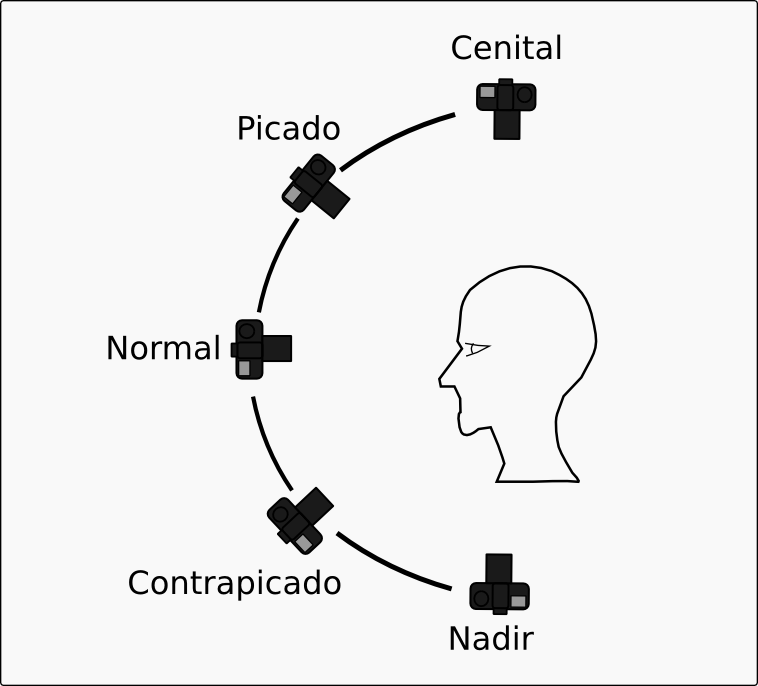
\includegraphics[width=6cm]{otros/manual/angulos.png}}
	\caption{Ángulos posibles}
	\label{mec:angulos}
\end{figure}

\begin{itemize}
	\item \textbf{Juego de lucha uno contra uno o \textit{1v1}}: Implica que dos personajes con exactamente las mismas capacidades, acciones posibles y atributos competirán en el mismo entorno. En lo que a la competición se refiere no existe ninguna entidad más involucrada por lo que el factor decisivo a la hora de determinar un ganador serán las habilidades de quien sea que controle a los personajes.
	\item \textbf{Top-Down}: Vista que en videojuegos se puede referir tanto a un plano cenital\footnote{En fotografía, el punto de vista de la cámara se encuentra perpendicular al suelo} como a un plano picado\footnote{En fotografía, el punto de vista de la cámara tiene un ángulo superior a 45 grados pero sin llegar a 90 con respecto al suelo}, se pueden ver ejemplos en la figura \ref{mec:angulos}. En el presente caso se utiliza un \textbf{plano picado}.
	\item \textbf{En dos dimensiones}: Pues el contenido del videojuego son imágenes planas dibujadas para representar los diferentes estados de los personajes, en ningún momento se utiliza ningún modelo entres dimensiones.
\end{itemize}

\subsection{Agente}

Agente se define como algo capaz de percibir el entorno mediante \textbf{sensores} y actuar sobre el mismo en consecuencia mediante \textbf{actuadores}\cite{modern}. En este sentido, en presente proyecto tanto los sensores como los actuadores formarán parte del software, es decir, no se materializan en ningún objeto físico.

\bigskip

Se entiende \textbf{\textit{percept}} o \textbf{percepto} como las entradas percibidas por en agente en un instante determinado. En general, la elección de una acción solo puede depender de las percepciones observadas hasta la fecha y no de entradas o estados que no hayan sido observados.

\bigskip

EL comportamiento se define en la \textbf{\textit{función del agente}} que es la encargada de generar una acción para el estado o secuencia de estados presentados. La implementación más sencilla, y suficientemente capaz en algunos casos, es la creación manual de una tabla que considere una serie de estados para los cuales tiene definida una acción.

\bigskip

Mientras que la función del agente es una representación externa, el programa que la implementa internamente se conoce como \textbf{\textit{programa del agente}}. A este programa nos referiremos con frecuencia simplemente como \textbf{agente}.

\bigskip

El entorno que se presenta al agente en este proyecto será de índole \textbf{competitiva} ya que su intención será maximizar su medida de \textbf{rendimiento} lo que implicará de forma efectiva minimizar la de su contrincante.

\subsection{Conexión entre ambos}

Muy comúnmente se necesitan implementar comportamientos complejos en el entorno de un videojuego. Sin embargo la aproximación utilizada en prácticamente todos los casos es determinar un árbol de comportamiento que no implica aprendizaje. Esto aporta la capacidad de modificar a un personaje fácilmente por parte de los diseñadores, pudiendo estar seguros de que las acciones tomadas siempre serán las planeadas por ellos. 

\bigskip

En busca de una experiencia que presente un desafío pero sin hacerlo injusto para el jugador, esta ha probado ser la mejor elección. Sin embargo, se está desaprovechando la utilización de este tipo de aplicaciones para ayudar a avanzar al campo de la inteligencia artificial. Además, podría dar lugar a una serie de videojuegos con mecánicas muy interesantes donde elementos del entorno sean capaces de aprender de los jugadores.

\bigskip

Pese a que sí existen videojuegos que aportan la posibilidad de agregar un agente que los controle, con mucha frecuencia se están presentando entornos demasiado simples o que no se benefician de usar técnicas de IA complejas. En este proyecto se aborda la creación de un videojuego que balancea entre la simplicidad y complejidad necesarias para que un agente pueda aprender sobre él sin ser capaz de determinar una estrategia óptima en todos los casos, todo esto mientras se muestra un entorno interesante y competitivo a un jugador humano.



\section{Objetivos}

El objetivo global es implementar un videojuego que contenga a un agente capaz de controlar a uno de los personajes simulando un comportamiento competitivo. Más concretamente los sub-objetivos a abarcar son los siguientes:

\begin{enumerate}
	
	{\item {\bf Implementar el videojuego:}
		Se necesita una plataforma que permita tanto a un jugador humano como al agente interactuar con el entorno del videojuego siguiendo ambos las reglas que este mismo define.
	}

	{\item {\bf Implementar el agente con las técnicas escogidas:}
		Se requiere realizar la implementación del agente para simular un comportamiento competitivo.
	}

	{\item {\bf Realizar el entrenamiento del agente:}
		Se necesitará ejecutar un proceso de entrenamiento para que este adquiera la información necesaria para comportarse adecuadamente en el entorno competitivo del juego.
	}

	{\item {\bf Obtener datos sobre las capacidades del agente:}
		Se deberán obtener datos sobre el comportamiento del agente en el entorno del juego al competir con otras posibles implementaciones del mismo que no incluyan el uso de técnicas de inteligencia artificial.
	}

	{\item {\bf Analizar los resultados obtenidos:}
		Se recopilará la información obtenida durante las etapas del proyecto y se realizará un análisis que resuma lo que ha logrado el agente.
	}
	
\end{enumerate}

\section{Organización del documento}

La finalidad de este documento es presentar cómo se han resuelto los objetivos definidos para el proyecto. Para ello se explicarán las diferentes partes que forman el producto final así como las tareas que han sido realizadas a lo largo del proyecto y que han dado lugar al mismo tal y como se presenta.

\begin{itemize}
	\item El \textbf{\textit{capítulo 2}} introduce al videojuego y a las implementaciones realizadas, así como el algoritmo utilizado, la otra implementación del agente y las técnicas de entrenamiento.
	\item El \textbf{\textit{capítulo 3}} contiene tanto el análisis de requisitos del proyecto como las diferentes partes que definen el alcance del mismo.
	\item El \textbf{\textit{capítulo 4}} documenta las etapas de gestión del proyecto que contienen: gestión de riesgos, gestión de la configuración, metodología empleada, planificación temporal, análisis de costes y plan de comunicaciones.
	\item En el \textbf{\textit{capítulo 5}} se introducen las partes de la aplicación especificando su arquitectura así como las herramientas utilizadas para su creación.
	\item Es en el \textbf{\textit{capítulo 6}} donde se puede ver la documentación asociada al diseño de implementación del producto final con los diagramas asociados.
	\item El \textbf{\textit{capítulo 7}} contiene las pruebas que verifican y validan el sistema.
	\item En el \textbf{\textit{capítulo 8}} se recogen las conclusiones obtenidas una vez finalizado el proyecto así como las posibles ampliaciones futuras que serían de utilidad.
	\item Finalmente, se agregan dos \textbf{\textit{apéndices}} que contienen el manual técnico y manual de usuario.
\end{itemize}



